\documentclass{bioinfo}
\copyrightyear{2013}
\pubyear{2013}
\usepackage{url}

\begin{document}
\firstpage{1}

\title[ADAM: Cloud Scale Genomic Processing]{ADAM: A Data Format And Pipeline For Cloud Scale Genomic Processing}
\author[Massie \textit{et~al}]{Matt~Massie\,$^{1,*}$, Frank~Austin~Nothaft\,$^{1,*}$, Christopher~Hartl\,$^{2}$, Christos~Kozanitis\,$^1$,
Andr\'{e}~Schumacher\,$^3$, Timothy~Danford\,$^4$, Carl~Yeksigian\,$^4$, Jey~Kottalam\,$^1$, Anthony~D.~Joseph\,$^1$,
and David~Patterson$\,^1$\footnote{to whom correspondence should be addressed}}
\address{$^{1}$Department of Electrical Engineering and Computer Science, University of California, Berkeley\\
$^{2}$The Broad Institute of MIT and Harvard\\
$^{3}$International Computer Science Institute (ICSI), University of California, Berkeley\\
$^{4}$GenomeBridge, Cambridge, MA}

\history{Received on XXXXX; revised on XXXXX; accepted on XXXXX}

\editor{Associate Editor: XXXXXXX}

\maketitle

\begin{abstract}

\section{Motivation:}
Current genomics data formats and processing pipelines are not designed to scale well to large datasets. As the quantity of genetic
data continues to increase, it is desirable to be able to process this data in the cloud. We introduce a new set of file formats that are
designed for cloud computing and that replace the BAM and VCF standards.

\section{Results:} On a high coverage~(60$\times$) 250GB NA12878 BAM file, we are able to perform Sorting and Duplicate Marking in under
50 minutes on 100 node cluster. On a single node, we are twice as fast as Picard and Samtools. ADAM files are up to 25\% smaller than
their equivalent BAM files.

\section{Availability:}
The ADAM project website is at \url{http://adam.cs.berkeley.edu}. ADAM is open source under the Apache 2 license, is deployed through Maven,
and the source is available through GitHub.

\section{Contact:} \href{massie@berkeley.edu}{\{massie,fnothaft,pattrsn\}@berkeley.edu}
\end{abstract}

\section{Introduction}
\label{sec:introduction}

The Sequence/Binary Alignment/Map~(SAM/BAM) and Variant Call Format~(VCF) file formats were designed before multi-node processing
and cloud computing were in vogue---thusly, they were designed for single node processing~\citep{li09}. As noted by \citet{mcpherson09}, as
next generation sequencing~(NGS) methods continue to improve, the latency of alignment and variant calling is becoming increasingly costly
for scientists who are using genomics in a clinical setting, or who are working on very large datasets. To address this issue, it is desirable to be
able to compute on genomic data across many machines, but characteristics of the BAM and VCF file formats practically limit scalability to 8
nodes~\citep{niemenmaa12}.

As the scalability limitations are inherent to the file formats\footnote{This is discussed in more detail in \S\ref{sec:approach}.}, we
choose to rethink file formats for genomics, instead of looking to incrementally improve either BAM or VCF. We view the following
points as critical design questions:

\begin{itemize}
\item BAM and VCF optimize for row-oriented, flat file access. Is this access pattern the best pattern for genomics?
\item Scientists want to process data from many different programming languages. How can we avoid incompatibilities between
data processed using different languages or libraries?
\item Genomic data will be processed on various computing systems, including single workstations, large dedicated clusters,
and using cloud computing services. How can we jointly optimize for these diverse platforms?
\item The file formats we use must be flexible enough to support new fields, but should not become disorganized. Is there a better
way to support this extensibility than attribute maps?
\end{itemize}

To address these problems, we introduce ADAM, a set of formats, APIs, and processing stage implementations for genomic data.
ADAM is fully open source under the Apache 2 license, and is implemented on top of Avro~\citep{avro} and Parquet~\citep{parquet}
for data storage. Our reference pipeline is implemented on top of Spark, a high performance in-memory map-reduce
system~\citep{zaharia10}. This combination provides the following advantages:

\begin{enumerate}
\item Avro provides explicit data schema access in C/C++/C\#, Java/Scala, Python, php, and Ruby;
\item Parquet allows efficient distributed access and use by database systems like Impala and Shark; and 
\item Spark improves performance through in-memory caching and reducing disk I/O.
\end{enumerate}

These changes lead to significant performance improvements, and improve the format's cross-platform portability. On a single
node, we are able to speedup sort and duplicate marking by 2$\times$. More importantly, on a 250 Gigabyte~(GB) high~(60$\times$) coverage
human genome, this system achieves a 50$\times$ speedup on a 100 node computing cluster, fulfilling the promise of scalability of ADAM.
We provide an extensive review of ADAM's performance in~\S\ref{sec:performance}.

The ADAM format provides explicit schemas for read and reference oriented~(pileup) sequence data, variants, and genotypes. As the
schemas are implemented in Apache Avro---a cross-platform/language serialization format---they eliminate
the need for the development of language-specific libraries for format decoding/encoding, which eliminates the possibility of library
incompatibilities. Additionally, any application that implements the ADAM schema is compatible with ADAM. This prevents
applications from being locked into a specific tool or pattern. The ADAM stack is inspired by the ``narrow waist'' of the Internet Protocol~(IP)
suite (see Figure~\ref{fig:stack-model}). We consider this stack model to be the greatest contribution of ADAM.

In this paper, we start by introducing why a new approach is necessary, and what our new approach is in~\S\ref{sec:approach}. We review the
design and performance of our pipeline in~\S\ref{sec:methods} and~\S\ref{sec:performance}. Finally, we provide a comprehensive comparison of
ADAM against other data formats and discuss the future growth of ADAM in~\S\ref{sec:discussion}.

\section{Approach}
\label{sec:approach}

As we noted in the introduction, instead of trying to extend the BAM and VCF file formats, we choose to reimagine these formats. We choose
to reimagine BAM and VCF because we feel that these file formats are too limiting. This knowledge comes from several attempts to adapt the
BAM and VCF file formats for distributed processing~\citep{niemenmaa12}. These adaptations have been limited in their ability to scale to larger
cluster sizes due to several issues intrinsic to BAM and VCF:

\begin{itemize}
\item BAM and VCF both depend on centralized headers, which must be globally distributed; and
\item BAM and VCF both have irregular record sizes, which limits the efficiency of row-parallel reading. 
\end{itemize}

These characteristics limit the performance of applications that are performing parallel access to all records of a BAM or VCF file. However,
this points at another severe problem in bioinformatics: modern file formats lock users into a single processing platform or technique. There are
several reasons that traditional flat file formats are not ideal for genomics. Several important access patterns that are difficult to implement on a flat,
row-oriented file include:

\begin{itemize}
\item \textbf{Database Queries:} Extending BAM to provide standard database queries required a significant extension~\citep{kozanitis13}.
No such extension exists for VCF data.
\item \textbf{Efficient Predication:} Typically, a user would only like to process certain records. Currently, for both BAM and VCF, a user must load all
records and then perform a filter, which is inefficient. BAM supports the inclusion of an index file~(BAM Index, BAI), but this index file accelerates
to a minor subset of filtering patterns\footnote{Typically, the first step of variant calling involves a filter that removes low quality reads. These filters
are based on position-independent data~(e.g. mapping quality, boolean flags) and cannot be accelerated with the BAI.}.
\item \textbf{Projection of Specific Fields:} It is typical for an application to only read some fields of a BAM record across all records, especially for
statistics collection tools like SAMtools' \texttt{flagstat}~\citep{li09}. Row-oriented formats like BAM and VCF cannot support these access patterns.
\end{itemize}

Moving forward, we seek to meet two major goals: we want to provide an extensible architecture that will allow for efficient future extension of the
file format, and we want to provide an initial implementation of that architecture that addresses the problems introduced above. In the remainder
of this section, we review our high-level architecture that provides extensibility, and then we provide a technical overview of our reference pipeline.

\subsection{Architectural Overview}
\label{sec:architectural-overview}

The primary takeaway from our criticisms of BAM and VCF are that the formats are difficult to specialize for certain processing patterns without
changing the implementation of the formats themselves. This issue is similar to the problems addressed during the development of the Open
Systems Interconnection~(OSI) model and Internet Protocol~(IP) stack for networking services~\citep{zimmermann80}. Specifically, the developers
of the OSI model and the IP stack needed to make many different technologies and systems function in unison---to do this, they introduced the
concept of a ``narrow waist,'' which guaranteed that a new protocol or technology would be compatible with the rest of the system if it implemented
one specific interface.

We draw significant inspiration from the development of networking standards---we believe that our largest contribution is the introduction of a
stack model for genomics, where the explicit ADAM schema is the ``narrow waist'' in our stack. This allows components to be cleanly
interchanged as long as they implement the ADAM schema. Our stack is pictured in Figure~\ref{fig:stack-model}.

\begin{figure}[h]
\begin{center}
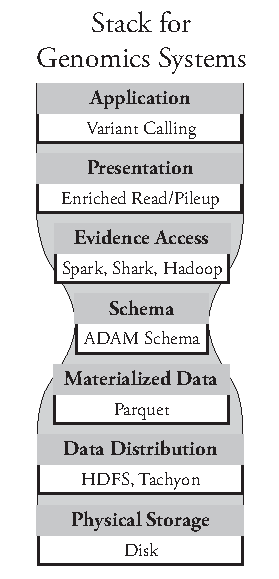
\includegraphics[width=0.4\linewidth]{stack-model.pdf}
\end{center}
\caption{A Stack Model for Genomics}
\label{fig:stack-model}
\end{figure}

The seven layers of our stack model are decomposed as follows, traditionally numbered from bottom to top:

\begin{enumerate}
\item {\bf Physical Storage:} This layer coordinates data writes to physical media, usually magnetic disk.
\item {\bf Data Distribution:} This layer manages access, replication, and distribution of the genomics files that have been written to disk.
\item {\bf Materialized Data:} This layer encodes the patterns for how data is encoded and stored. This provides read/write efficiency
and compression.
\item {\bf Data Schema:} This layer specifies the representation of data when it is accessed, and forms the narrow waist of the pipeline.
\item {\bf Evidence Access:} This layer implements efficient methods for performing common access patterns such as random database
queries, or sequential/parallel reading of records from a flat file.
\item {\bf Presentation:} The presentation layer provides the application developer with efficient and
straightforward methods for querying the characteristics of individual portions of genetic data.
\item {\bf Application:} Applications like variant calling and alignment are implemented in this layer.
\end{enumerate}

A well defined software stack has several significant advantages. By limiting application interactions with layers lower than the presentation layer,
application developers are given a clear and consistent view of the data they are processing. By divorcing the API from the data
access layer, we unlock significant flexibility. With careful design in the data format and data access layers, we can seamlessly
support conventional flat file access patterns, while also allowing easy access to data with database methods. By treating the
compute substrate and storage as separate layers, we also drastically increase the portability of the APIs that we implement. 

\subsection{Reference Implementation}
\label{sec:reference-implementation}

In this paper, we present a reference implementation of a read processing pipeline~(\texttt{adam-core}). This implementation is fully open source
and is designed for a distributed, in-memory map-reduce framework. 

\begin{methods}
\section{Methods}
\label{sec:methods}

ADAM contains formats for storing read and reference oriented sequence information, and variant/genotype data.
The read oriented sequence format is forwards and backwards compatible with BAM/SAM, and the variant/genotype
data is forwards and backwards compatible with VCF. We provide two APIs:

\begin{enumerate}
\item A data format/access API implemented on top of Apache Avro and Parquet
\item A data transformation API implemented on top of Apache Spark
\end{enumerate}

In this section, we provide brief introductions to these two APIs. We then introduce the data representations, discuss the content
of each representation, and introduce the transforms that we provide for each representation.

\subsection{Data Format and Schema}
\label{sec:data-format-and-schema}

The data representation for the ADAM format is described using the open source Apache Avro data serialization
system~\citep{avro}. The Avro system also provides a human readable schema description language that can
auto-generate the schema implementation in several common languages including C/C++/C\#, Java/Scala, php,
Python, and Ruby. This flexibility provides a significant cross-compatibility advantage over the BAM/SAM format,
where the data format has only been implemented for C/C++ through Samtools~\citep{li09} and for Java through
Picard~\citep{picard}. Additionally, there are known incompatibilities between these two implementations.

We layer this data format inside of the Parquet~\citep{parquet} column store. Parquet is an open source columnar storage
format that was designed by Cloudera and Twitter. It can be used as a single flat file, a distributed file, or as a database inside of Hive, Shark, or Impala. Columnar stores provide significant compression~\citep{abadi06}, and are a very good match for genomics access patterns.

Figure~\ref{fig:file-format} shows how ADAM in Parquet compares to BAM. We remove the file header from BAM,
and instead distribute these values across all of the records stored. This dissemination eliminates global information and makes the file much
simpler to distribute across machines. This distribution is effectively free in a columnar store, as the store just notes that the information is
replicated across many reads. Parquet achieves additional data parallelism by writing data to disk in regularly sized row groups\footnote{This
allows for parallelism across both rows and columns.}.

\begin{figure}[h]
\begin{center}
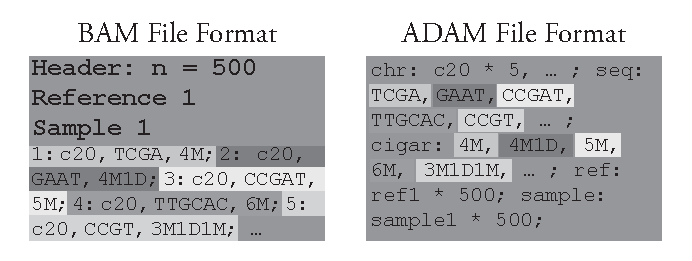
\includegraphics[width=\linewidth]{file-format.pdf}
\end{center}
\caption{Comparative Visualization of BAM and ADAM File Formats}
\label{fig:file-format}
\end{figure}

The data types presented in this section make up the narrow waist of our proposed genomics stack in Figure \ref{fig:stack-model}. We provide
the following datatypes:

\begin{itemize}
\item \textbf{ADAMRecord:} This datatype is for storing read data, and provides similar semantics to the read storage in SAM/BAM;
\item \textbf{ADAMPileup:} This datatype stores reference-oriented pileup data, broken out by individual read base;
\item \textbf{ADAMGenotype:} This datatype represents the genotype of a single chromosome of a single sample; and
\item \textbf{ADAMVariant:} This datatype represents a single variant allele which segregates at a site.
\end{itemize}

A full description of the fields of the data types is available in the ADAM technical report~\citep[see][\S5]{massie13}. We note that the internal
representations of the data may change at any point in time---for the most up to date schema, we refer readers to the ADAM repository.

\subsection{Data Transformations}
\label{sec:data-transformations}

In this section, we provide a brief discussion of the transforms and utilities implemented inside of ADAM. For an extended description of
the \textit{Sorting}, \textit{Mark Duplicates}, \textit{BQSR}, and \textit{Indel Realignment} algorithms, we refer readers to the appendix of
\citet{massie13} which discusses these algorithms in more detail.

\end{methods}

\section{Performance}
\label{sec:performance}

Table~\ref{tab:overview} previews the performance of ADAM for \textit{Sort} and \textit{Mark Duplicates}.

\begin{table}[h]
\processtable{\textit{Sort} and \textit{Mark Duplicates} Performance on NA12878\label{tab:overview}}
{\begin{tabular}{ l c c }
\toprule
\bf Software & \bf EC2 profile & \bf Wall Clock Time \\
\midrule
Picard 1.103 & 1 \texttt{hs1.8xlarge} & 17h 44m \\
ADAM 0.5.0 & 1 \texttt{hs1.8xlarge} & 8h 56m \\
ADAM 0.5.0 & 32 \texttt{cr1.8xlarge} & 33m \\
ADAM 0.5.0 & 100 \texttt{m2.4xlarge} & 21m \\ 
\midrule
\bf Software & \bf EC2 profile & \bf Wall Clock Time \\
\midrule
Picard 1.103 & 1 \texttt{hs1.8xlarge} & 20h 22m \\
ADAM 0.5.0 & 100 \texttt{m2.4xlarge} & 29m \\
\botrule
\end{tabular}}{}
\end{table}

By using dictionary coding, run length encoding with bit-packing, and GZIP compression, ADAM files can be stored using less
disk space than an equivalent BAM file. Typically, ADAM is up to 75\% of the size of the compressed BAM for the
same data. If one is performing pileup aggregation, compression can improve to over 50\%.

\section{Discussion}
\label{sec:discussion}

\begin{table}[h]
\processtable{Comparison of File Formats\label{tab:comparison}}
{\begin{tabular}{ l c c }
\toprule
 & \bf BAM & \bf ADAM \\
\midrule
\bf Size & 1.0$\times$ & 0.75-0.9$\times$ \\
\bf Scalability & $<$8 machines & $>$100 machines \\
\midrule
& \bf VCF & \bf ADAM \\
\midrule
\bf Scalability & $<$8 machines & $>$100 machines \\
\botrule
\end{tabular}}{}
\end{table}

\subsection{Dedicated Clusters vs. Cloud Computing}
\label{sec:dedicated-clusters-vs-cloud-computing}

ADAM is designed to fit all computing platforms well.

\section{Conclusion}
\label{sec:conclusion}

This paper presents ADAM, a new data storage format and processing pipeline for genomics data. 

ADAM makes use of efficient columnar storage systems to improve the lossless compression available
for storing read data, and uses in-memory processing techniques to eliminate the read processing bottleneck faced
by modern genomics pipelines. On top of the file formats that we have implemented, we also present APIs that enhance
developer access to read, pileup, genotype, and variant data. 

We are currently in the process of extending ADAM to support SQL querying of genomic data, and extending our transformations API
to more programming languages. 

ADAM promises to improve the development of applications that process genomic data, by removing current difficulties with the extraction
and loading of data and by providing simple and performant programming abstractions for processing this data.

\section*{Acknowledgement}
\label{sec:acknowledgement}

The authors would like to thank their many colleagues who provided feedback on early implementations of ADAM, and on drafts of the
manuscript.

\paragraph{Funding\textcolon}
\label{sec:funding}

This research is supported in part by NSF CISE Expeditions award CCF-1139158 and DARPA XData Award FA8750-12-2-0331, a NSF
Graduate Research Fellowship (\textbf{FIXME}) and gifts from Amazon Web Services, Google, SAP,  Apple, Inc., Cisco, Clearstory Data,
Cloudera, Ericsson, Facebook, GameOnTalis, General Electric, Hortonworks, Huawei, Intel, Microsoft, NetApp, Oracle, Samsung, Splunk,
VMware, WANdisco and Yahoo!.

\bibliographystyle{natbib}

\bibliography{adam-ismb-2013}

\end{document}
